\chapter{Proposed System Design}
The design of \textbf{Event Blinker} adheres to contemporary software engineering principles, prioritizing decoupling, horizontal scalability, and high data integrity. The system is architected as a three-tier ecosystem where spatial relationships, real-time states, and intelligent reasoning are unified.

\section{System Architecture and Orchestration}
The architecture follows a distributed service-oriented design, ensuring that logical domains—such as identity management and spatial processing—remain independent and maintainable. This allows the system to scale its computational resources independently based on user demand.

\begin{figure}[H]
    \centering
    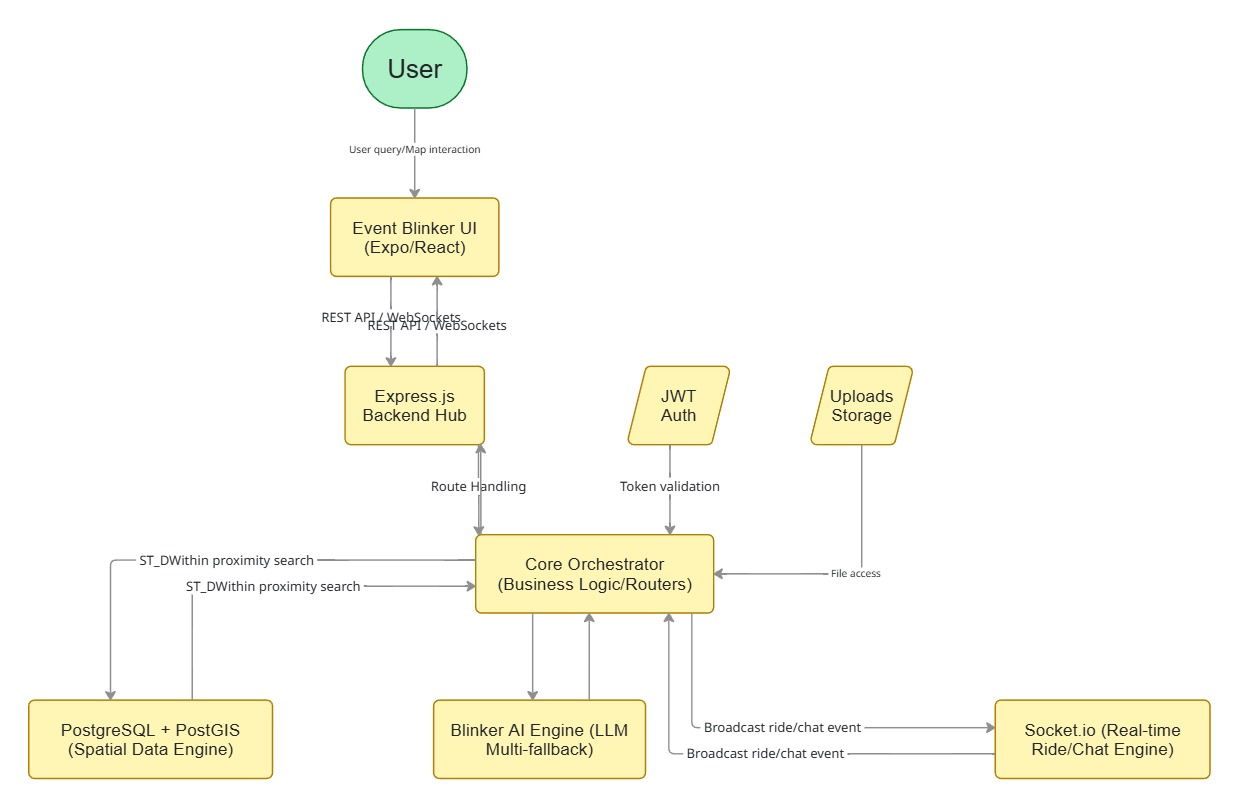
\includegraphics[width=0.9\textwidth]{system_archi.jpg}
    \caption{System Architecture: Three-Tier Decoupled Ecosystem for Urban Discovery}
    \label{fig:archi_final_v2}
\end{figure}

\begin{figure}[H]
    \centering
    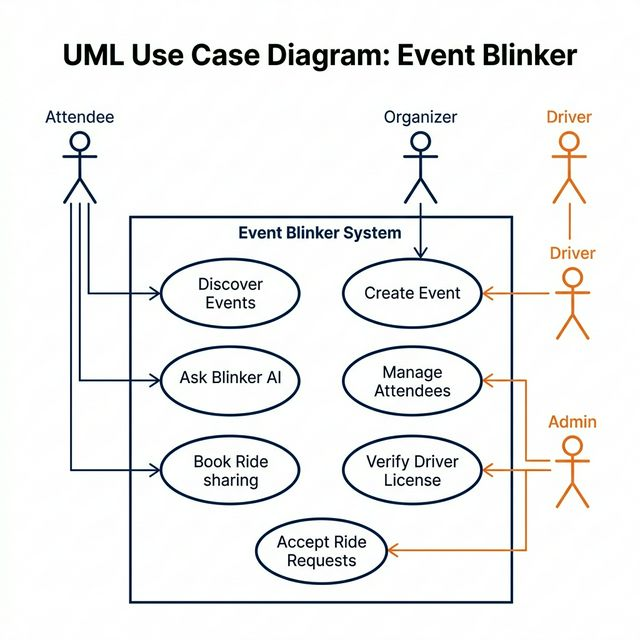
\includegraphics[width=0.85\textwidth]{use_case.png}
    \caption{Project Use Case Diagram: Interactions between Attendees, Riders, and Organizers.}
    \label{fig:use_case_main}
\end{figure}

The architecture is divided into several specialized layers, each responsible for a distinct part of the event-to-commute lifecycle.

\subsection{Presentation Layer: Multi-Client Infrastructure}
The presentation layer serves as the primary interaction point for the three main stakeholder groups of the platform: Attendees, Riders, and Organizers.

\subsubsection{Attendee Mobile Application (React Native)}
The Attendee app is the core of the discovery experience. It is built using the React Native framework to ensure cross-platform compatibility while maintaining native-level performance. The interface is centered around an interactive map (Mapbox GL), which dynamically updates based on the user's viewport. It handles complex states such as AI chat interactions, ride request broadcasts, and event detail visualization.

\subsubsection{Rider Interface and Verification}
The Rider interface is specialized for mobility providers. It includes features for real-time bid submission, GPS tracking, and identity documentation upload. The interface is designed for high-contrast visibility to ensure safety during transit operations.

\begin{figure}[H]
    \centering
    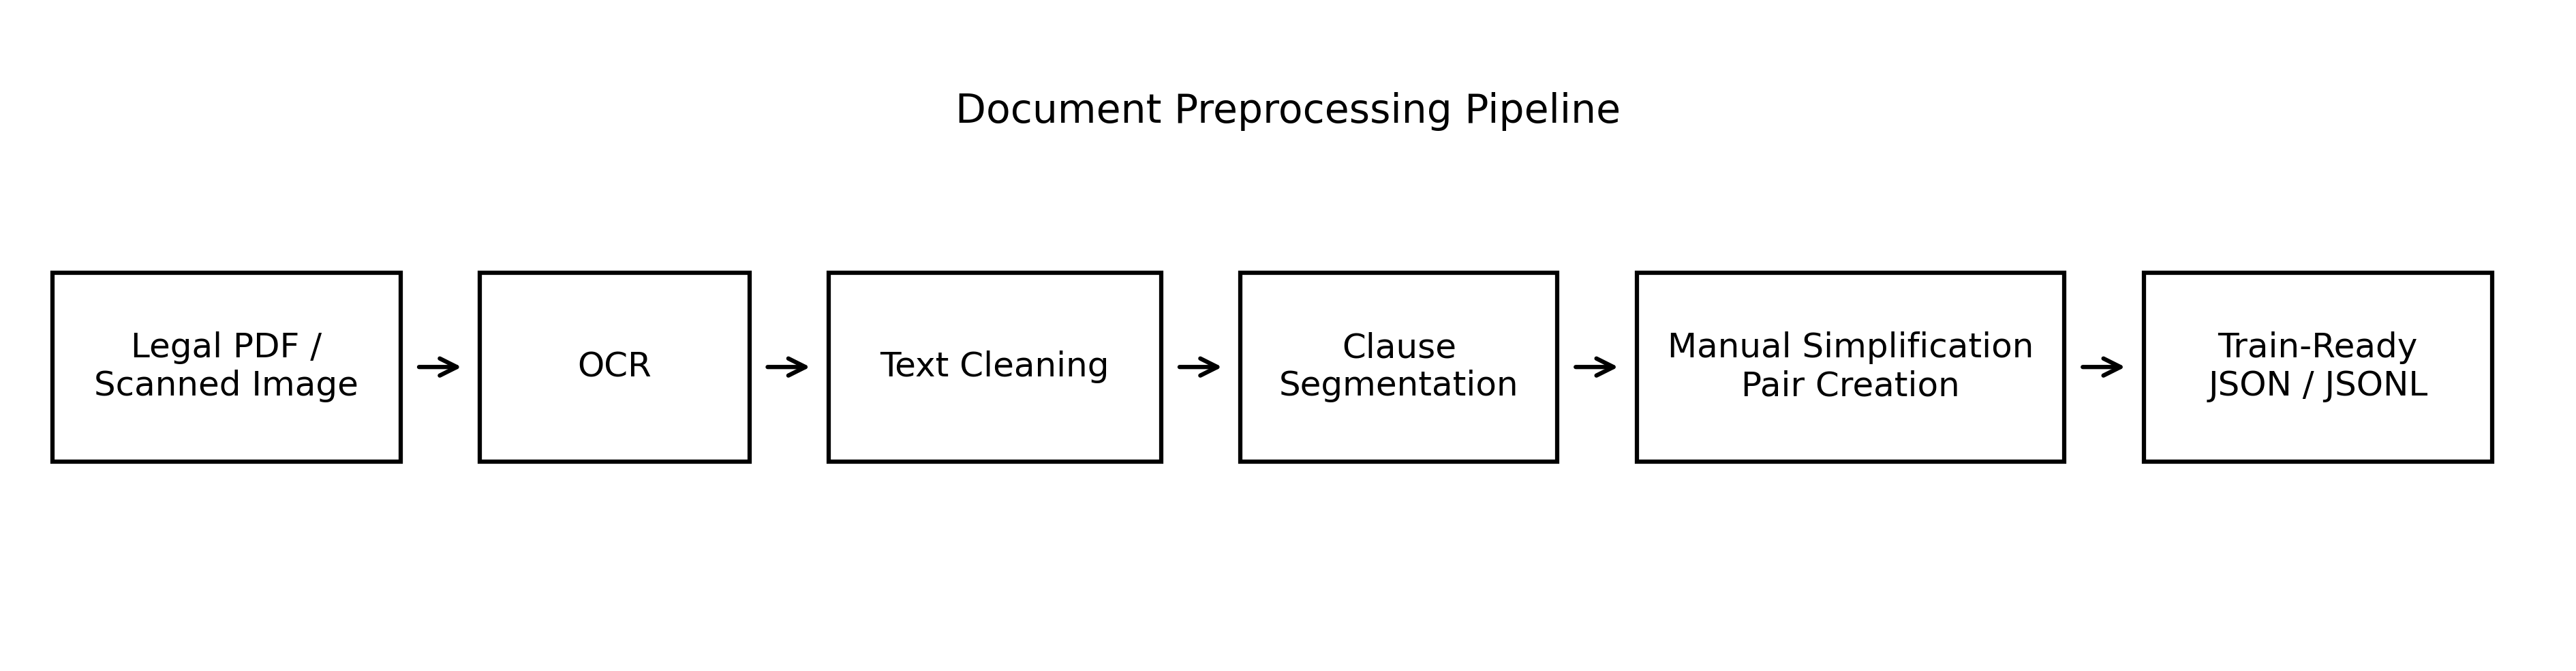
\includegraphics[width=0.92\textwidth]{preprocessing_pipeline.png}
    \caption{Document Verification Pipeline: Rider Upload, Admin Queue, Verification, and Status Activation.}
    \label{fig:verification_pipeline}
\end{figure}

\subsubsection{Administrative and Organizer Portals}
The system includes two web-based dashboards built with React.js. The \textbf{Organizer Portal} allows event creators to manage listings and view engagement analytics. The \textbf{Admin Portal} is a high-privilege interface used for global governance, specifically the verification of rider identity documents (KYC).

\subsection{Application Layer: Backend Logic and AI}
The application layer is the "intelligence" of the system, orchestrating data flow between the clients and the persistence layer.

\subsubsection{Node.js API Gateway}
The backend is implemented using Node.js and Express.js, providing a non-blocking, asynchronous environment suitable for high-concurrency urban surges. The API is structured into modular routers (e.g., \texttt{authRouter}, \texttt{eventRouter}, \texttt{rideRouter}) to ensure maintainability.

\subsubsection{Geospatial Discovery Module}
This module interface with PostGIS to perform spatial operations. It handles the translation of mobile GPS coordinates into SRID-compliant geometric points and executes the radial search queries that power the event discovery map.

\subsubsection{Real-Time Synchronization Engine (Socket.io)}
For features requiring sub-100ms latency—such as live chat and ride bidding—the system uses WebSockets. This bypasses the overhead of standard HTTP requests, allowing for a "push-based" update model where the server notifies clients of new bids or message events instantly.

\subsubsection{Support Assistant Logic}
A lightweight assistant is integrated into the application layer to provide context-aware support for venue-specific queries. The assistant is grounded via a Retrieval-Augmented Generation (RAG) strategy. When a query is received, the backend retrieves relevant relational metadata from PostgreSQL and injects it into the prompt. This ensures that responses are grounded in the actual facts of the platform rather than the model's training data.

\begin{figure}[H]
    \centering
    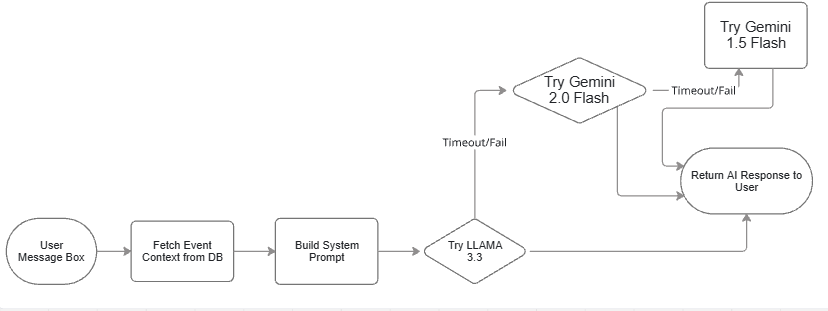
\includegraphics[width=0.88\textwidth]{ai.png}
    \caption{Support Assistant Architecture: Internal prompt engineering and knowledge retrieval workflow.}
    \label{fig:ai_grounding_diag}
\end{figure}

\begin{figure}[H]
    \centering
    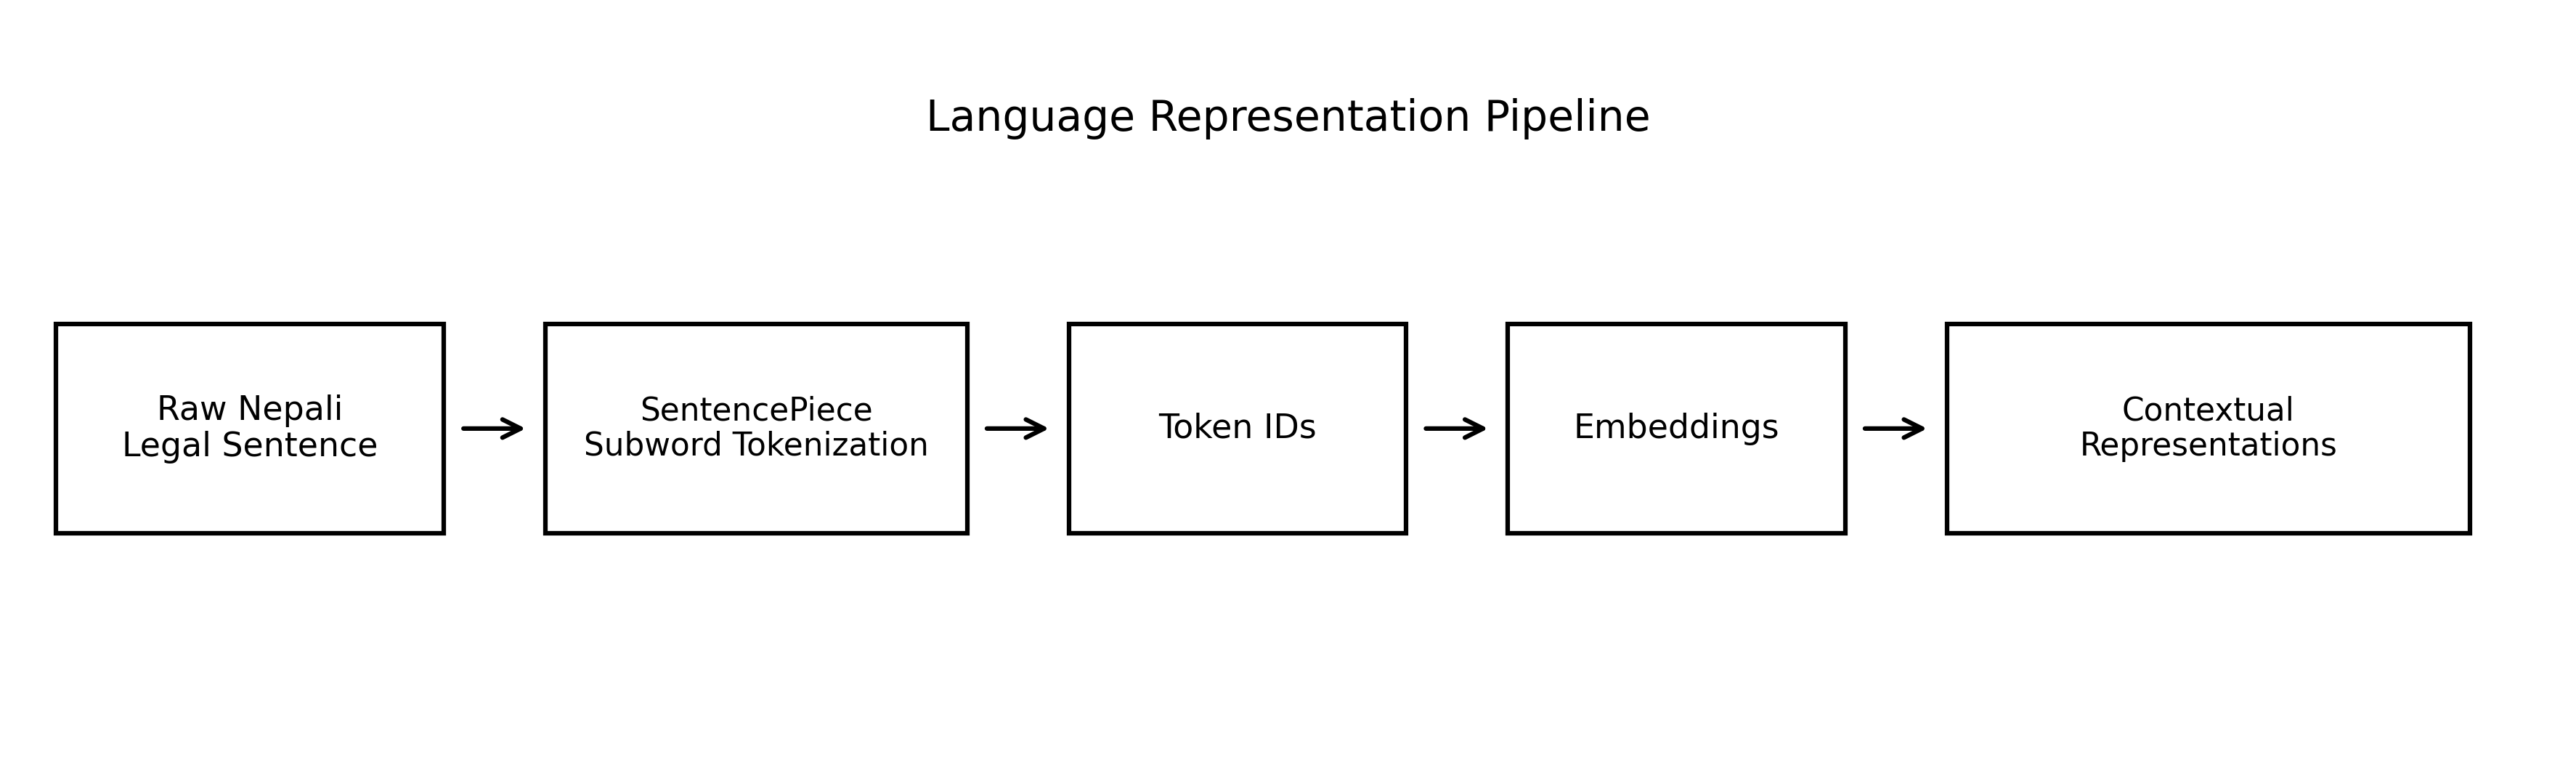
\includegraphics[width=0.92\textwidth]{language_representation_pipeline_fixed.png}
    \caption{Language representation and reasoning pipeline for the support assistant.}
    \label{fig:language_representation}
\end{figure}

\subsection{Data Layer: Spatial Persistence}
The data layer ensures the integrity and durability of all platform information.

\subsubsection{Relational Metadata (PostgreSQL)}
Standard relational data—such as user profiles, transaction logs, and rid-offer histories—are stored in PostgreSQL. We utilize foreign key constraints and ACID transactions to ensure that financial and identity data remain consistent.

\subsubsection{Spatial Data (PostGIS)}
The complex geometric data representing event venues and user locations are stored using the PostGIS extension. This allows us to perform high-performance spatial joins and proximity filters that would be impossible with a standard relational store.

\section{System Requirements Modeling}
To ensure the system meets both user expectations and technical constraints, we have defined a comprehensive set of requirements.

\subsection{Functional Requirements (FR)}
The following core functionalities define the platform's operational capabilities:
\begin{itemize}
    \item \textbf{FR-1: Geospatial Event Discovery}: The system must provide a map interface where events are visualized based on user proximity.
    \item \textbf{FR-2: Integrated Support Assistant}: Users must be able to resolve venue-specific queries through a support assistant grounded in platform factuality.
    \item \textbf{FR-3: P2P Ride-Sharing Lifecycle}: The system must support the complete ride-sharing cycle: request $\rightarrow$ bid $\rightarrow$ acceptance $\rightarrow$ completion.
    \item \textbf{FR-4: Multi-Role Verification}: Administrators must have an interface to verify rider identity documents (License/Billbook).
    \item \textbf{FR-5: Event Engagement Analytics}: Organizers must be able to track attendee interest and event performance.
\end{itemize}

\subsection{Non-Functional Requirements (NFR)}
To ensure a professional user experience, the system adheres to strict performance thresholds:
\begin{itemize}
    \item \textbf{NFR-1: Spatial Latency}: Viewport-aware spatial queries must execute in sub-100ms intervals to ensure map fluidity.
    \item \textbf{NFR-2: Real-time Concurrency}: The Socket.io layer must support concurrent active connections without messaging delay.
    \item \textbf{NFR-3: Data Integrity}: Sensitive user documents and credentials must be managed using AES-256 encryption and stateless JWT tokens.
    \item \textbf{NFR-4: Platform Resilience}: The system must implement robust failover strategies to ensure overall service availability during surges.
\end{itemize}

\section{Interaction Workflow and Lifecycle}
The integration of ride-sharing and event discovery is defined by a sequential state machine. This ensures that the system state is always predictable and synchronized across all clients.

\subsubsection{The Unified User Journey}
The workflow begins with \textbf{Discovery}, where the user explores the map. Upon finding an event, the user enters the \textbf{Engagement} phase, interacting with the AI or event details. If the user decides to attend, they enter the \textbf{Mobility} phase, triggering the ride-sharing workflow.

\subsubsection{The Ride-Bidding State Machine}
\begin{enumerate}
    \item \textbf{Intent}: User clicks the "Book Commute" button on an event detail page.
    \item \textbf{State Initialization}: The system initializes a \texttt{ride\_request} record, automatically setting the destination to the event's geometric \texttt{GEOMETRY:Point}.
    \item \textbf{Broadcast}: A WebSocket event \texttt{ride:new\_request} is broadcast to the group of verified riders within the vicinity.
    \item \textbf{Bidding}: Riders submit bids (fare offers). The user views these real-time offers in a list.
    \item \textbf{Finalization}: Upon user acceptance, the system transitions to \texttt{ride:accepted}, initializing a private chat room for the trip.
\end{enumerate}

\section{Detailed Data Schema}
The database layer uses UUID v4 for all primary identifiers to ensure distributed uniqueness across the ecosystem. The schema is normalized to the 3rd Normal Form (3NF) to prevent data redundancy.

\begin{table}[H]
\centering
\caption{Detailed Technical Table Schemas and Data Domains}
\label{tab:db_detailed_schema}
\small
\begin{tabularx}{\textwidth}{@{}lXp{6cm}@{}}
\toprule
\textbf{Table Domain} & \textbf{Logical Purpose} & \textbf{Key Technical Columns} \\
\midrule
\texttt{users} & Verified Identity & \texttt{id}, \texttt{email}, \texttt{password\_hash}, \texttt{user\_type} \\
\texttt{events} & Geospatial Knowledge & \texttt{location\_geom}, \texttt{organizer\_id}, \texttt{category} \\
\texttt{riders} & Mobility Provider & \texttt{verification\_status}, \texttt{license\_url}, \texttt{vehicle\_id} \\
\texttt{ride\_requests} & Mobility Transaction & \texttt{pickup\_geom}, \texttt{destination\_geom}, \texttt{status} \\
\texttt{ride\_offers} & Real-time Bidding & \texttt{ride\_id}, \texttt{rider\_id}, \texttt{offered\_fare} \\
\texttt{chats} & Communication & \texttt{room\_id}, \texttt{sender\_id}, \texttt{message\_content} \\
\bottomrule
\end{tabularx}
\end{table}



